%%% cs269.tex
%%%
%%% This LaTeX source document can be used as the basis for your technical
%%% paper or abstract. Intentionally stripped of annotation, the parameters
%%% and commands should be adjusted for your particular paper - title, 
%%% author, article DOI, etc.
%%% The accompanying ``template.annotated.tex'' provides copious annotation
%%% for the commands and parameters found in the source document. (The code
%%% is identical in ``template.tex'' and ``template.annotated.tex.'')

\documentclass[conference]{acmsiggraph}

\TOGonlineid{45678}
\TOGvolume{0}
\TOGnumber{0}
\TOGarticleDOI{1111111.2222222}
\TOGprojectURL{}
\TOGvideoURL{}
\TOGdataURL{}
\TOGcodeURL{}

\title{Methods in Segmented Image Seam Carving}

\author{
  Weiss, Tomer\\
  \texttt{tweiss@cs.ucla.edu}
  \and
  Liu, Brian\\
  \texttt{liubrian7@ucla.edu}
}



\pdfauthor{Robert A. Smith}

\keywords{Image resizing, Image retargeting, Image seams, Content-aware image manipulation, Display devices}

\begin{document}

%% \teaser{
%%   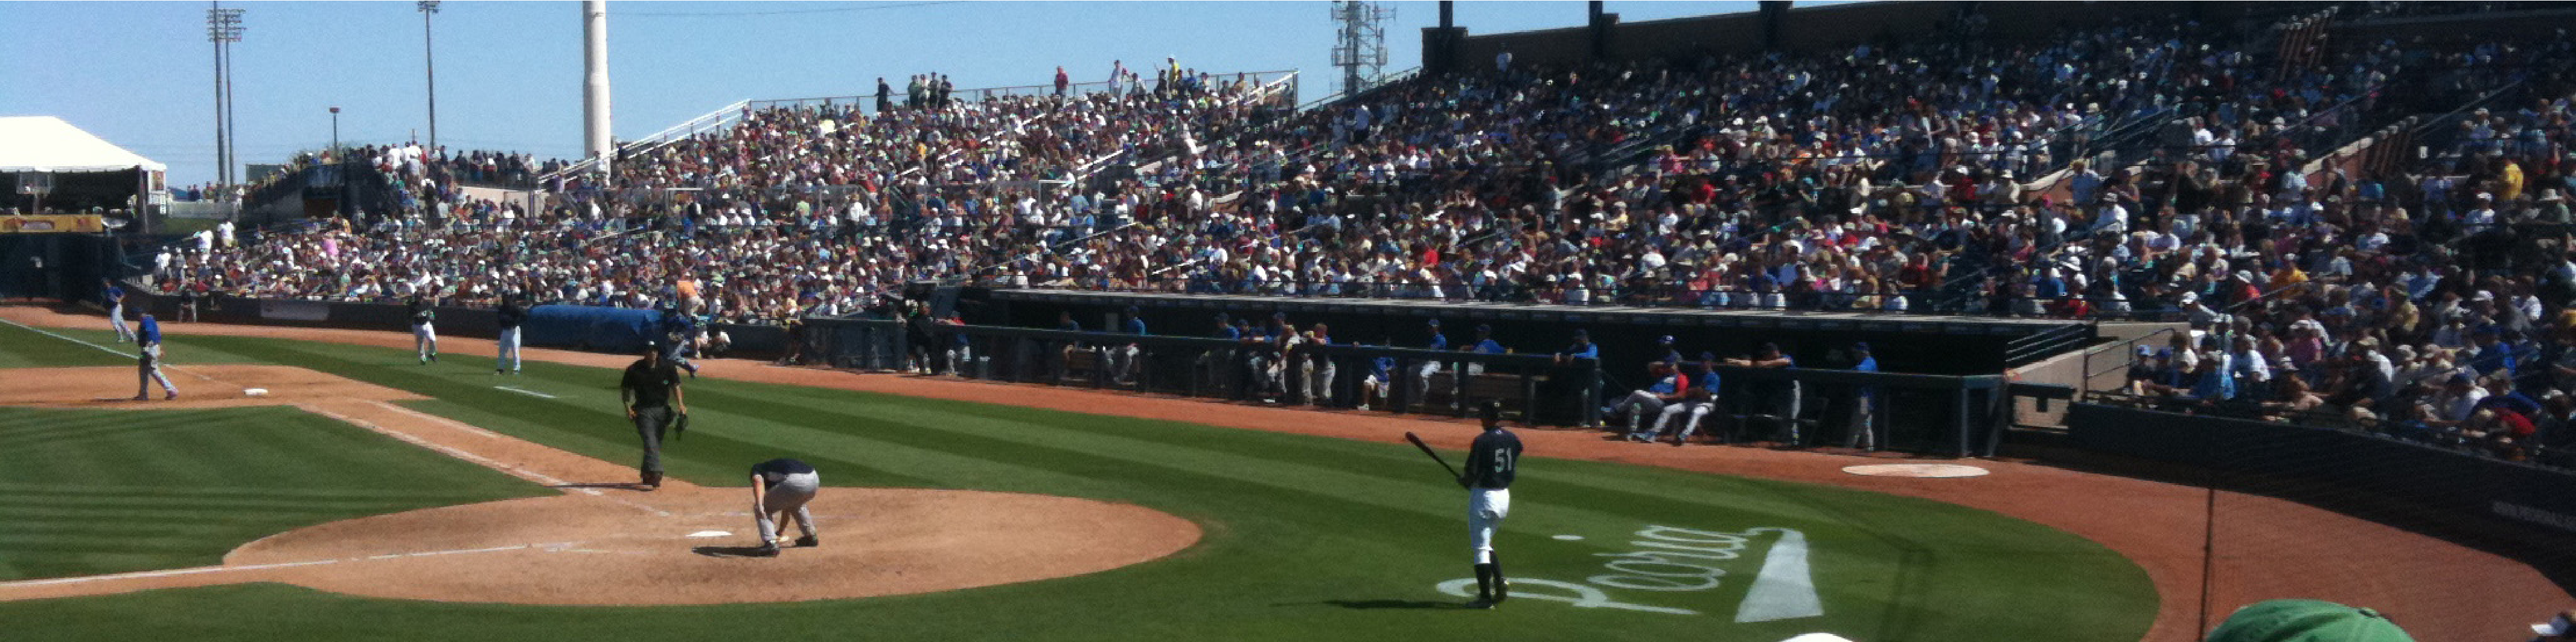
\includegraphics[height=1.5in]{images/sampleteaser}
%%   \caption{Spring Training 2009, Peoria, AZ.}
%% }

\maketitle

\begin{abstract}

Seam carving deals with the task of taking an input picture and resizing it to fit another screen type and aspect ratio. In this paper, we discuss possible methods to improve the algorithm, and also make it work faster. We approached this problem using the segmentation approach, and got promising results.

 % %Citations can be done this way~\cite{Liu2007} or this more % % %concise 
 % %way~\shortcite{Liu2007}, depending upon the application.

%%Ut wisi enim ad minim veniam, quis nostrud exerci tation ullamcorper
%%suscipit lobortis nisl ut aliquip ex ea commodo consequat. Duis autem
%%vel eum iriure dolor in hendrerit~\cite{Pellacini:2005:LAH}
%%in vulputate velit esse molestie~\cite{notes2002} 
%%consequat, vel illum dolore eu feugiat nulla facilisis at vero eros et
%%accumsan et iusto odio dignissim qui blandit praesent luptatum zzril
%%delenit augue duis dolore te feugait nulla facilisi.~\cite{Park:2006:DSI}

\end{abstract}

\begin{CRcatlist}  

  \CRcat{I.3.0}{Computing Methodologies}{Computer Graphics—General}  
  
  \CRcat{I.4.10}{Computing Methodologies}{Image Processing And Computer Vision}{Image Representation};     
  
\end{CRcatlist}

\keywordlist

%% Use this only if you're preparing a technical paper to be published in the 
%% ACM 'Transactions on Graphics' journal.

\TOGlinkslist

%% Required for all content. 

\copyrightspace

\section{Introduction}

With the recent advances in imaging technology, digital images have become an important component of media distribution. Images are frequently used in news stories, and people post their pictures online to be seen by family and friends. Images, however, are typically authored once, but need to be adapted for consumption under varied conditions. As an example, pictures are often displayed on different screens, where the area available for the picture may have a different aspect ratio than the original image has for layout reasons. Dynamically changing the layout of web pages in browsers should take into account the distribution of text and images, resizing them if necessary. The use of thumbnails that faithfully represent the image content is important in image browsing applications. In addition, a variety of displays can be used for image viewing, ranging from high-resolution computer monitors to TV screens and low-resolution mobile devices. This diversity of image consumption conditions introduces a new problem: images must be resized for optimal
display or use in different applications. The process, also known as image re-targeting or image resizing, consists of modifying the image’s aspect ratio and size in order to best satisfy the new requirements. However,
straightforward image resizing operators, such as scaling, often do not produce satisfactory results, since they are oblivious to image content. To overcome this limitation, a class of techniques attempt to resize the images in a content-aware fashion, i.e., taking the image content into consideration to preserve important regions and minimize distortions. This is a challenging problem, as it requires preserving the relevant information while maintaining an aesthetically pleasing image for the user.

One of those techniques is Seam Carving, where the general idea is to decrease the image width (or height) one pixel at a time, by removing a seam of minimal importance. A seam is defined as an 8-connected path of pixels (from top to bottom, or from left to right of the image, depending on which dimension is being reduced) that contains only one pixel per row (or column). When the importance map is based on gradient energy, the first removed seam will be in a homogeneous area. The image is then readjusted by shifting pixels left or up to compensate for the removed
seam, resulting in an image which is one pixel smaller, either on width or height. So the image changes only at the seam region, while the other areas remain intact. 

In the original paper, the optimal seams are computed using dynamic programming, and an algorithm for resizing in both dimensions by choosing between optimal vertical or horizontal seams is also presented. The technique can be used for enlarging the image, by finding seams to be removed and duplicating them. It produces impressive results when there are enough low-importance seams to be removed, but creates distortions and artifacts when seams cut through important areas.

Motivated by the compelling applications and the challenges related to the problem, we proposed to use image segmentation to improve the seam carving algorithm. There are other methods that rely on segmentation to assign saliencies to different regions in the image. Previous work by ~\cite{Liu2007} and ~\cite{Hasan2009} suggests to segment the image into regions and then assign saliencies to each region by considering heuristics such as the region size, position in the image, and relationships between neighboring regions. ~\cite{Setlur2005} proposed to segment the image using mean-shift and assign saliencies to the obtained regions by a combination of bottom-up and top-down features. Also, ~\cite{Avidan2007} ,authors of the original Seam Carving algorithm, suggested that users could scribble on salient areas. 

To summarize, our goal is to experiment with different combinations of Seam Carving and image segmentation, and by so to improve the results of the original paper.


\section{Technical details}

\subsection{Overview}

Our method builds upon the basis of the original seam carving algorithm, where we the laplacian to find the energy levels of each pixel in the input image. After finding the energy levels, we segment the image to smaller, mini pictures in a grid like fashion -- vertical or horizontal. For example, if we segment the image to 3 by 3 segments, then the we get a total of 9 segments. On each such segment we engage the next step of the seam carving algorithm -- i.e. finding the seams. This step is done via the basic dynamic algorithm for finding seams, but on each segment separately.

\subsection{Image Energy}
Our initial approach, similar to the original paper, is to preserve the image's energy, by removing unnoticeable pixels. That leads to the following energy function that was used in the original paper:

\begin{equation}
e_I(I)=   \lvert \frac{\partial}{\partial x} I \rvert + \lvert  \frac{\partial}{\partial y} I 
\rvert 
\end{equation}

we need a resizing operator that will be less restrictive than cropping or column removal, but can preserve the image content better than single pixel removals. This leads to our strategy of seam carving and the definition of image seams. Let $I$ be and $n x m $ image and define a vertical seam to be:

\begin{equation}
s^{x} = { \left\{ s_{i}^{x} \right\}  }_{i=1}^{n} = 
{\left\{ (x(i),i) \right\}}_{i=1}^{n} ,s.t. \forall i \lvert x(i) - x(i - 1)  \rvert \leq 1
\end{equation}

where x is a mapping $x : [1, . . . , n] \longrightarrow [1, . . . , m]$. That is, a vertical seam is an 8-connected path of pixels in the image from top to bot-tom, containing one, and only one, pixel in each row of the image. Similarly, if y is a mapping y : [1, . . . , m] → [1, . . . , n], then a horizontal seam is:

\begin{equation}
s^{y} = { \left\{ s_{j}^{y} \right\}  }_{j=1}^{m} = 
{\left\{ (y(j),j) \right\}}_{j=1}^{m} ,s.t. \forall j \lvert y(j) - y(j - 1)  \rvert \leq 1
\end{equation}

The pixels of the path of seam $s$ (e.g. vertical seam $\left\{ s_{i} \right\}$ ) will therefore be $I_s = {\left\{ (I(s_i) \right\}}_{i=1}^{n} = {\left\{ I{ (x(i),i)) \right\}}_{i=1}^{n} $ . Note that similar to the removal of a row or column from an image, removing the pixels of a seam from an image has only a local effect: all the pixels of the image are shifted left (or up) to compensate for the missing path.




\subsection{Dynamic Programming Algorithm}
We find the optimal seam for each segment using dynamic programming. The first step is to traverse the image from the second row to the last row and compute the cumulative minimum energy $M$ for all possible connected seams for each entry $(i, j)$:

At the end of this process, the minimum value of the last row in $M$ will indicate the end of the minimal connected vertical seam. Therefore, in the second step we backtrack from this minimum entry on $M$ to find the path of the optimal seam. The definition of $M$ for horizontal seams is similar:

\begin{equation}
M(i,j) = e(i,j) + min( M(i-1,j-1), M(i-1,j), M(i-1,j+1) )
\end{equation}

We repeat the above process for each segment, and then remove the newly found seams for each of them, hence resizing the picture.

\subsection{Runtime}
Running the Seam Carving algorithm on each segment separately, we achieved an improvement in runtime. First, let us remember that finding $s$ seams takes $o(s m n)$ in the original method, where $m,n$ define the image's size and $s$ is the number of seams.
With our segmented approach running on a single thread, the runtime time is equal to the total number of segments multiplied by the running time for each segment. So, for:
$s_m = # of segments in m, e.g. 2 in naive example$
$s_n = # of segments in n, e.g. 2 in naive example$
$Total # of segments = s_m*s_n (4 in naive example)$
$Total # of seams in each segment  = s/(s_m*s_n) (s/4 in naive example
Dimension of segmented =  m*n/(s_m*s_n) ( m*n / 4 in naive)$
$Total Running time for each segment = O( s*m*n / ((s_m*s_n)^2) ) (naive $ example: O (s*m*n / 16))

$Total running time of each segment serially = (s_m*s_n) * O( s*m*n / ((s_m*s_n)^2) ) 
O( (s*m*n)/(s_m*s_n) ) naive example: 4 * O (s*m*n/16) = O(s*m*n/4) - when run serially$
When run concurrently we can achieve speed increases up to O(s*m*n/16) ?



\subsection{Implementation}





\section{Exposition}

Lorem ipsum dolor sit amet, consectetur adipisicing elit, sed do
eiusmod tempor incididunt ut labore et dolore magna aliqua. Ut enim ad
minim veniam, quis nostrud exercitation ullamco laboris nisi ut
aliquip ex ea commodo consequat. Duis aute irure dolor in
reprehenderit in voluptate velit esse cillum dolore eu fugiat nulla
pariatur. Excepteur sint occaecat cupidatat non proident, sunt in
culpa qui officia deserunt mollit anim id est laborum.

\begin{equation}
 \sum_{j=1}^{z} j = \frac{z(z+1)}{2}
\end{equation}

\begin{eqnarray}
x & \ll & y_{1} + \cdots + y_{n} \\
  & \leq & z
\end{eqnarray}

Lorem ipsum dolor sit amet, consectetur adipisicing elit, sed do
eiusmod tempor incididunt ut labore et dolore magna aliqua. Ut enim ad
minim veniam, quis nostrud exercitation ullamco laboris nisi ut
aliquip ex ea commodo consequat. Duis aute irure dolor in
reprehenderit in voluptate velit esse cillum dolore eu fugiat nulla
pariatur. Excepteur sint occaecat cupidatat non proident, sunt in
culpa qui officia deserunt mollit anim id est laborum.


Lorem ipsum dolor sit amet, consectetur adipisicing elit, sed do
eiusmod tempor incididunt ut labore et dolore magna aliqua. Ut enim ad
minim veniam, quis nostrud exercitation ullamco laboris nisi ut
aliquip ex ea commodo consequat. Duis aute irure dolor in
reprehenderit in voluptate velit esse cillum dolore eu fugiat nulla
pariatur. Excepteur sint occaecat cupidatat non proident, sunt in
culpa qui officia deserunt mollit anim id est laborum.
\begin{figure}[ht]
  \centering
  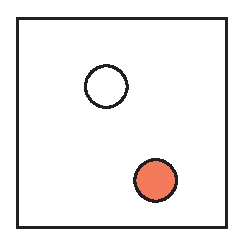
\includegraphics[width=1.5in]{images/samplefigure}
  \caption{Sample illustration.}
\end{figure}
Lorem ipsum dolor sit amet, consectetur adipisicing elit, sed do
eiusmod tempor incididunt ut labore et dolore magna aliqua. Ut enim ad
minim veniam, quis nostrud exercitation ullamco laboris nisi ut
aliquip ex ea commodo consequat. Duis aute irure dolor in
reprehenderit in voluptate velit esse cillum dolore eu fugiat nulla
pariatur. Excepteur sint occaecat cupidatat non proident, sunt in
culpa qui officia deserunt mollit anim id est laborum.

Lorem ipsum dolor sit amet, consectetur adipisicing elit, sed do
eiusmod tempor incididunt ut labore et dolore magna aliqua. Ut enim ad
minim veniam, quis nostrud exercitation ullamco laboris nisi ut
aliquip ex ea commodo consequat. Duis aute irure dolor in
reprehenderit in voluptate velit esse cillum dolore eu fugiat nulla
pariatur. Excepteur sint occaecat cupidatat non proident, sunt in
culpa qui officia deserunt mollit anim id est laborum.

Lorem ipsum dolor sit amet, consectetur adipisicing elit, sed do
eiusmod tempor incididunt ut labore et dolore magna aliqua. Ut enim ad
minim veniam, quis nostrud exercitation ullamco laboris nisi ut
aliquip ex ea commodo consequat. Duis aute irure dolor in
reprehenderit in voluptate velit esse cillum dolore eu fugiat nulla
pariatur. Excepteur sint occaecat cupidatat non proident, sunt in
culpa qui officia deserunt mollit anim id est laborum.

\section{Exposition}

Lorem ipsum dolor sit amet, consectetur adipisicing elit, sed do
eiusmod tempor incididunt ut labore et dolore magna aliqua. Ut enim ad
minim veniam, quis nostrud exercitation ullamco laboris nisi ut
aliquip ex ea commodo consequat. Duis aute irure dolor in
reprehenderit in voluptate velit esse cillum dolore eu fugiat nulla
pariatur. Excepteur sint occaecat cupidatat non proident, sunt in
culpa qui officia deserunt mollit anim id est laborum.

Lorem ipsum dolor sit amet, consectetur adipisicing elit, sed do
eiusmod tempor incididunt ut labore et dolore magna aliqua. Ut enim ad
minim veniam, quis nostrud exercitation ullamco laboris nisi ut
aliquip ex ea commodo consequat. Duis aute irure dolor in
reprehenderit in voluptate velit esse cillum dolore eu fugiat nulla
pariatur. Excepteur sint occaecat cupidatat non proident, sunt in
culpa qui officia deserunt mollit anim id est laborum.

Lorem ipsum dolor sit amet, consectetur adipisicing elit, sed do
eiusmod tempor incididunt ut labore et dolore magna aliqua. Ut enim ad
minim veniam, quis nostrud exercitation ullamco laboris nisi ut
aliquip ex ea commodo consequat. Duis aute irure dolor in
reprehenderit in voluptate velit esse cillum dolore eu fugiat nulla
pariatur. Excepteur sint occaecat cupidatat non proident, sunt in
culpa qui officia deserunt mollit anim id est laborum.

Lorem ipsum dolor sit amet, consectetur adipisicing elit, sed do
eiusmod tempor incididunt ut labore et dolore magna aliqua. Ut enim ad
minim veniam, quis nostrud exercitation ullamco laboris nisi ut
aliquip ex ea commodo consequat. Duis aute irure dolor in
reprehenderit in voluptate velit esse cillum dolore eu fugiat nulla
pariatur. Excepteur sint occaecat cupidatat non proident, sunt in
culpa qui officia deserunt mollit anim id est laborum.

Lorem ipsum dolor sit amet, consectetur adipisicing elit, sed do
eiusmod tempor incididunt ut labore et dolore magna aliqua. Ut enim ad
minim veniam, quis nostrud exercitation ullamco laboris nisi ut
aliquip ex ea commodo consequat. Duis aute irure dolor in
reprehenderit in voluptate velit esse cillum dolore eu fugiat nulla
pariatur. Excepteur sint occaecat cupidatat non proident, sunt in
culpa qui officia deserunt mollit anim id est laborum.

\section{Conclusion}

There is much future work to be done in the area of image resizing and Seam Carving. We didn't have enough time to investigate other methods to segment a picture, like image saliency as shown in  

Lorem ipsum dolor sit amet, consectetur adipisicing elit, sed do
eiusmod tempor incididunt ut labore et dolore magna aliqua. Ut enim ad
minim veniam, quis nostrud exercitation ullamco laboris nisi ut
aliquip ex ea commodo consequat. Duis aute irure dolor in
reprehenderit in voluptate velit esse cillum dolore eu fugiat nulla
pariatur. Excepteur sint occaecat cupidatat non proident, sunt in
culpa qui officia deserunt mollit anim id est laborum.

\section*{Acknowledgements}

To Robert, for all the bagels.

\bibliographystyle{acmsiggraph}
\bibliography{template}
\end{document}
